
\section{Experimental results}
\label{sec:experimental-results}
% <<<<<<< HEAD
% \begin{table}[t]
%   \centering
%   \twocolumn[

%   \begin{@twocolumnfalse}
%     \caption{Benchmark programs using \texttt{delay} constructs} \label{table:benchmark}
%     \scalebox{0.85}{
%       \begin{tabular}{|c| c | c | c | c | c | c | c |}
% 	\cline{4-8}
% 	\multicolumn{3}{c|}{}											& HRTCS 		& Motor 		  & Robot 			  & AECS/CD1  		   & AECS/CD2\\ \hline
% 	\multirow{12}{*}{JOP} 		& \multicolumn{2}{|c|}{BCRT} 		&0.0334 ms 		& 0.0361 ms		  & 0.0325 ms		  & 0.1683 ms		   & 0.1881 ms\\ \cline{2-8}   
%         & \multicolumn{2}{|c|}{WCRT} 		&0.1120 ms 		& 0.1116 ms		  & 0.0601 ms		  & 0.7147 ms		   & 1.0115 ms\\ \cline{2-8} 
%         & \multirow{2}{*}{Delay 1}	 & M..N &50.3-200.3 ms 	& 2.4-7.4772 ms	  & 1230-2274.0263 ms & 10000-42473.2197 ms& 10000-53772.0045 ms \\ \cline{3-8} 
%         &			   & d			 		&1506-1787  	& 67 			  & 37861			  & 59427		       &53160\\ \cline{2-8}
%         & \multirow{2}{*}{Delay 2}	 & M..N & 	N/A 		& 1.667-5.2452 ms & N/A				  & N/A 			   &10000-53772.0045 ms\\ \cline{3-8} 
%         &			   & d			 		& 	N/A	 		& 47			  & N/A				  & N/A       		   &53160\\ \cline{2-8}
%         & \multirow{2}{*}{Delay 3}	 & M..N & 	N/A	 		& 0.05-0.2232 ms  & N/A				  & N/A       		   &N/A\\ \cline{3-8} 
%         &			   & d			 		& 	N/A	 		& 2		      	  &	N/A				  & N/A       		   &N/A\\ \cline{2-8}
%         & \multirow{2}{*}{Delay 4}	 & M..N & 	N/A	 		& 0.3-1.0044 ms   & N/A				  &	N/A       		   &N/A\\ \cline{3-8} 
%         &			   & d				 	& 	N/A	 		& 9				  & N/A				  &	N/A      		   &N/A\\ \cline{2-8}
%         & \multirow{2}{*}{Delay 5}	 & M..N & 	N/A	 		& 0.733-2.3436 ms & N/A				  &	N/A      		   &N/A\\ \cline{3-8} 
%         &			   & d			 		& 	N/A	 		& 21 			  &	N/A				  & N/A      		   &N/A\\ \hline
% 	\multirow{12}{*}{TP-JOP} 	& \multicolumn{2}{|c|}{BCRT} 		&0.0028 ms 		& 0.0060 ms		  & 0.0011 ms		  & 0.0532 ms		   & 0.0292 ms\\ \cline{2-8}   
%         & \multicolumn{2}{|c|}{WCRT} 		&0.0329 ms 		& 0.0393 ms		  & 0.0361 ms		  & 0.5072 ms		   & 0.8388 ms\\ \cline{2-8} 
%         & \multirow{2}{*}{Delay 1}	 & M..N &50.3-600.3 ms 	& 2.4-15.6265 ms  & 1230-42317.8276 ms& 10000-95358.8578 ms& 10000-287757.9834 ms \\ \cline{3-8} 
%         &			   & d			 		&18209-18232 	& 398 			  & 1171429			  & 188015		       &343054\\ \cline{2-8}
%         & \multirow{2}{*}{Delay 2}	 & M..N & 	N/A 		& 1.667-10.8757 ms& N/A				  & N/A 			   &10000-287757.9834 ms\\ \cline{3-8} 
%         &			   & d			 		& 	N/A	 		& 277			  & N/A				  & N/A       		   &343054\\ \cline{2-8}
%         & \multirow{2}{*}{Delay 3}	 & M..N & 	N/A	 		& 0.05-0.3534 ms  & N/A				  & N/A       		   &N/A\\ \cline{3-8} 
%         &			   & d			 		& 	N/A	 		& 9		      	  &	N/A				  & N/A       		   &N/A\\ \cline{2-8}
%         & \multirow{2}{*}{Delay 4}	 & M..N & 	N/A	 		& 0.3-1.9631 ms   & N/A				  &	N/A       		   &N/A\\ \cline{3-8} 
%         &			   & d				 	& 	N/A	 		& 50			  & N/A				  &	N/A      		   &N/A\\ \cline{2-8}
%         & \multirow{2}{*}{Delay 5}	 & M..N & 	N/A	 		& 0.733-4.79 ms   & N/A				  &	N/A      		   &N/A\\ \cline{3-8} 
%         &			   & d			 		& 	N/A	 		& 122 			  &	N/A				  & N/A      		   &N/A\\ \cline{2-8}
% 	\hline
%       \end{tabular}
%     }
%   \end{@twocolumnfalse}
%   ]

% \end{table}
% In this section, we present a set of SystemJ benchmark programs in which
% real-time requirements should be met.  We have carried out a set of
% experiments to obtain BCRT and WCRT of the benchmark programs on two
% execution platforms called Java Optimized Processor(JOP)
% \cite{jop:jnl:jsa2007} and TP-JOP \cite{6119095}. JOP is a hardware
% implementation of the JVM which enables real-time execution of Java
% programs by translating Java bytecodes into a sequence of JOP's native
% instructions called \emph{microcode} which is time-predictable. As
% SystemJ's default compilation target is Java source code, JOP is an
% excellent platform which enables us to analyze timing properties of
% SystemJ program. On the other hand, there is also an option where
% compiled code could be more tightly coupled to specific platforms such
% as TP-JOP, which execute SystemJ's kernel statements more
% efficiently. By utilizing our internal tools in conjunction with
% Worst-Case-Execution-Time (WCET) analyzer \cite{jop:jnl:jsa2007}
% provided by JOP tools, we were able to estimate BCRT and WCRT of our
% benchmark programs: (full-name?) HRTCS, Stepper motor controller (Motor)
% \cite{}, Robot and Access Environment Control System (AECS) \cite{}.

% % HRTCS, as already illustrated in Section \ref{sec:intr-motiv}, tests
% % for an ability of one's responsiveness by generating green lights
% % between the real-time range \emph{M - N}. For AECS \ref{} we have
% % replaced the external timer with our delay constructs. Stepper motor
% % controller is originally introduced in \cite{Bourke2009a} which
% % converted into SystemJ.

% As one can see in Table \ref{table:benchmark}, BCRT and WCRT of overall
% programs are smaller when they run on TP-JOP. For example, WCRT and BCRT
% of HRTCS are \(\times\)11.9 and \(\times\)3.4 smaller, respectively, for
% TP-JOP (0.0028, 0.0329 ms) compared to JOP (0.0334, 0.1120 ms). On the
% other hand, required logical delays \emph{d} are generally bigger on
% TP-JOP e.g. \(\times\)4.5 - \(\times\)5.9 and \(\times\)30.9 in Motor
% and Robot respectively. It is expected as their BCRT and WCRT
% differences are bigger on TP-JOP.  This also led to greater increase in
% minimum upper real-time bounds \emph{N} for TP-JOP in every example.  In
% AECS, there are two clock-domains using delay constructs that each has
% their own BCRT and WCRT. Again, individual BCRT and WCRT is smaller
% whereas \emph{d} is bigger on TP-JOP. One important property to note
% here, is that BCRT and WCRT of any clock-domains are invariant of
% \emph{d} as explained in Section \ref{sec:intr-real-time}. It is our
% fundamental assumption to find \emph{d} in our benchmark programs.
% =======

{\renewcommand{\arraystretch}{0.9}
\begin{table}[t]
	\small
	\centering
	\caption{An overview of the benchmark programs}
	\label{fig:benchlist}
	\scalebox{0.9}{
		\begin{tabular}{llp{0.5cm}p{1cm}}
\toprule
\emph{Benchmark}       & \emph{Delay constructs used in each CD} & \emph{\# of CDs} & 
\emph{Lines of code}        
\\ \midrule
HRTCS                  & \texttt{delay(50.3..200.3 ms)} ($CD1$) & 2                  & 56
\\ \midrule
\multirow{5}{*}{Motor} & \texttt{delay(2.4..2.4 ms)}        & \multirow{5}{*}{1} & \multirow{5}{*}{116} \\ 
											 & \texttt{delay(1.667..1.667 ms)}      &                    &                      \\ 
											 & \texttt{delay(0.05..0.05 ms)}       &                    &                      \\ 
											 & \texttt{delay(0.3..0.3 ms)}        &                    &                      \\ 
											 & \texttt{delay(0.733..0.733 ms)}      &                    &
\\ \midrule
\multirow{3}{*}{Printer}
& \texttt{delay(2.7..10.6 ms)} ($CD1$)      & \multirow{3}{*}{2}        & \multirow{3}{*}{39} \\
& \texttt{delay(1.2..30.3 ms)} ($CD2$)		  &														&											\\
& \texttt{delay(5.6..100.2 ms)} ($CD2$)     &														&											
\\ \midrule
\multirow{2}{*}{AECS} & \texttt{delay(10000 ms)} ($CD1$) 
& \multirow{2}{*}{2} & \multirow{2}{*}{267} \\
& \texttt{delay(10000..10000 ms)} ($CD2$) & &
\\ \bottomrule
\end{tabular}
}
\vspace{-20pt}
\end{table}
}

{\renewcommand{\arraystretch}{0.6}
\begin{table}[t]
\twocolumn[
\centering
\begin{@twocolumnfalse}
	\caption{Actual delays obtained for \texttt{delay} constructs in the
benchmark programs based on their BCRT and WCRT}
\label{fig:comparison}
\begin{tabular}{ c c l l l l l l }
	\toprule
	\multicolumn{2}{c}{} & \emph{HRTCS} & \emph{Motor} & \emph{Printer/CD1} &
	\emph{Printer/CD2} & \emph{AECS/CD1} &	\emph{AECS/CD2} \\ 
	\midrule
	\multicolumn{2}{c}{\emph{BCRT}}	& 0.0334 ms	& 0.0361 ms & 0.009613 ms &
	0.0263 ms & 0.1683 ms & 0.1881 ms\\ 
	\cmidrule(r){1-8}
	\multicolumn{2}{c}{\emph{WCRT}} &0.1120 ms & 0.1116 ms & 0.0603 ms
	& 0.0491 ms & 0.8148 ms & 1.0115 ms\\ 
	\cmidrule(r){1-8}

	\multirow{2}{*}{Delay 1} & M..N & 50.3-200.3 ms	& 2.4-8.4882 ms	  &
	2.7-16.9378 ms & 1.2-30.3 ms & 10000-42483.2198 ms& 10000-53882.0045 ms \\
	\cmidrule(r){2-8}
	& d &1506-1888 & 68 & 281 & 46-617 & 59428 &53160\\ 
	\cmidrule(r){1-8}
	\multirow{2}{*}{Delay 2} & M..N & N/A & 1.668-5.2452 ms & N/A &
	5.6-100.2 ms & N/A &10000-53882.0045 ms\\ 
	\cmidrule(r){2-8}
	& d & N/A & 48 & N/A & 213-2041 & N/A &53160\\ 
	\cmidrule(r){1-8}
	\multirow{2}{*}{Delay 3} & M..N & N/A & 0.05-0.2232 ms & N/A & N/A & N/A
	&N/A\\ 
	\cmidrule(r){2-8}
	& d & N/A & 2 & N/A & N/A & N/A &N/A\\ 
	\cmidrule(r){1-8}
	\multirow{2}{*}{Delay 4} & M..N & N/A & 0.3-1.0044 ms & N/A & N/A & N/A
	&N/A\\ 
	\cmidrule(r){2-8}
	& d & N/A & 9 & N/A & N/A & N/A &N/A\\ 
	\cmidrule(r){1-8}
	\multirow{2}{*}{Delay 5} & M..N & N/A & 0.833-2.3436 ms & N/A & N/A & N/A
	&N/A\\ 
	\cmidrule(r){2-8}
	& d & N/A & 21 & N/A
	& N/A & N/A &N/A\\ \bottomrule
\end{tabular}
\end{@twocolumnfalse}
]
\end{table}
}

We have carried out a number of experiments on a set of applications
with real-time constraints. The characteristics of the benchmark set
including required real-time delays and program sizes are shown in
Table~\ref{fig:benchlist}. 

HRTCS is the human response system described in
Section~\ref{sec:motivating-example}. AECS (Access and Environmental
Control System) is an application that controls an intelligent room
environment described in~\cite{aecs_ispa}.  The system interacts with
two external timers through input/output signals in order to measure how
long the entrance door to the room is being opened and time the illegal
presence (e.g. intruder) that is being detected. The program has been
modified such that the delay constructs are used instead of external
timers as shown in Figure~\ref{delaycode}. In the original AECS, the
system needed to trigger external timer by emitting the output signal in
order to wait for a specific amount of time (e.g.
\texttt{TimerTriggered} in Figure~\ref{delaycode:a}). When the timer
expires, it notifies back to the system through the input signal
\texttt{TimeOut} which is polled at the \texttt{await} statement. With
the new delay constructs, those timers are not necessary and delays can
be expressed directly in the code as shown in Figure~\ref{delaycode:b}.

\begin{figure}[h!]
	\begin{SubFloat}{\label{delaycode:a}}
		\centering
		\begin{minipage}[b]{0.3\linewidth}
			\scriptsize
\begin{verbatim}
emit TimerTriggered;
trap(T){
  abort(DoorOpened){
    await(TimeOut);
    exit(T); 
  }
}
\end{verbatim}
		\end{minipage}
	\end{SubFloat}
\hspace{1cm}%
	\begin{SubFloat}{\label{delaycode:b}}
		\centering
		\begin{minipage}[b]{0.5\linewidth}
			\scriptsize
\begin{verbatim}
// No emit statement
trap(T){
  abort(DoorOpened){
    delay(10000 ms);
    exit(T);  
  }
}
\end{verbatim}
		\end{minipage}
	\end{SubFloat}
\caption{Replacing external timer with delay construct}
\label{delaycode}
\end{figure}

Motor is a stepper motor controller from~\cite{Bourke2009a}, used for
producing monochrome images on paper by applying a correct application
of current to a print head (a row of resistors). In this example,
duration of current applied is controlled by the feedback logic using
real-time delays which are expressed in Esterel constructs. We have
rewritten the program in SystemJ and compared between desired and
relaxed delays according to WCRT and BCRT of the program. Printer is an
example from~\cite{Schneider:1999:CRT:555233}, which models a printer and
a spooler in timed CSP.  Their operation is rather simple: as soon as
the spooler receives a print job, passes it to the printer through a
channel where actual printing process take place. The example
demonstrates that by specifying delay bounds (e.g. 1 to 5 time units) on
receiving and sending channel ends data exchange will occur as soon as
both processes become ready.

%Robot is an industrial automation application that consists of two
%manufacturing belts and a robotic arm that splits goods according to
%their volumes. 

HRTCS consists of 2 CDs, but only one with real-time delays. AECS also
has 2 CDs; CD1 consist of a single delay statement, while CD2 has 2
delay statements. In this case, as explained previously, delay
statements replace the external timers and corresponding interface (I/O)
signals. The system triggers an alarm 10 seconds after detection of an
intruder or generates a beep sound when an entrance door is being opened
for the same amount of time. In Printer, each spooler and printer
process is mapped to a single clock-domain. Spooler CD sends a job to
the Printer CD between 2.7 to 10.6 ms after receiving it from the
enviornment (e.g. a user). On the other hand, Printer CD notifies
environment that it starts printing between 1.2 to 30.3 ms once it
receives the job from the Spooler CD. Actual print job is started
between 5.6 to 100.2 ms after the notification. In this example, bounded
delay ensures that both channel communication and print job should occur
within the specified amount of time. Lastly, Motor is a synchronous
program with 5 delay statements where they controls amount of current
into the stepper motor coils. 

%All these examples are written in
%the SystemJ language. The requirement to have deterministic or
%non-deterministic delays varies between each benchmark.  These delay
%requirements are shown in Table~\ref{fig:comparison} (\texttt{M..N}).


% In this section, we present a set of SystemJ benchmark programs in which
% real-time requirements should be met. We have carried out a set of
% experiments to obtain BCRT and WCRT of the benchmark programs on the
% execution platform called Java Optimized Processor(JOP)
% \cite{jop:jnl:jsa2007}. JOP is a hardware implementation of the JVM
% written in VHDL which enables real-time execution of Java programs by
% translating Java bytecodes into a sequence of JOP's native instructions
% called \emph{microcode} which is time-predictable. As SystemJ's default
% compilation target is Java source code, JOP is an excellent platform
% which enables us to analyze timing properties of SystemJ program.

% On the other hand, there is also an option where compiled code could be more
% tightly coupled to specific platforms such as TP-JOP, which execute SystemJ's
% kernel statements more efficiently.

We use the \textit{Java Optimized Processor}
(JOP)~\cite{jop:jnl:jsa2007}, to carry out all our experiments. JOP
implements the JVM specification in hardware directly, and has been
shown to be real-time amenable. We statically estimate the WCRT and BCRT
of these benchmark applications using the real-time analysis tools
provided by the JOP design framework. The \textit{Safety Critical Java}
(SCJ) specification we use for real-time analysis avoids garbage
collection (GC) and hence, GC overheads and unpredictability are
completely avoided. 

% We disable the \textit{Garbage Collector} (GC) in all experiments to
% avoid unwanted side-effects such as lengthening clock-domain logical
% tick times.

Table~\ref{fig:comparison} shows the result of our algorithm applied to
each benchmark program. Note that we allowed the compiler to relax the
upper real-time bounds even for bounded (\texttt{M..N}) or exact
(\texttt{M..M}) delays when it fails to find a feasible solution.
However, a user can prohibit this behavior through configuration that
such case is an error.

As a first step, BCRT and WCRT were calculated for all examples. Given
the real-time \mbox{\texttt{delay (M..N)}} provided by programmers,
required logical delay \textit{d} was determined by applying
Algorithm~\ref{alg:1}. In HRTCS, real-time delay of the range
50.3..200.3 (ms) is only satisfied when \emph{d} is between 1506 and
1787 (as shown previously in
Section~\ref{sec:intr-real-time}~\ref{sec:find-logic-delay}). Similarly,
Printer/CD2 satisfies real-time ranges of 1.2..30.3 (ms) and 5.6..100.2
(ms) when \emph{d} is 46..617 and 213..2041 respectively. It is then
compiler's job to statically choose one of the values in this range.

% The upper bound \texttt{N} needed to be relaxed for all examples other
% than HRTCS to obtain a feasible \texttt{d}. Therefore,
On the other hand, Algorithm \ref{alg:2} is applied to those examples,
where relaxation was required, to determine the minimum upper real-time
bound \emph{N} such that there exist a solution for \emph{D} in
Algorithm \ref{alg:1}. This algorithm gives a unique number for logical
tick delay \emph{d} such that \emph{d} = Min(\emph{$S_2$}) =
Max(\emph{$S_1$}). The compiler, therefore, will choose \emph{d} based
on the newly computed \emph{N} for the examples: Printer/CD1, Motor and
AECS.

\subsection{Improving results}

The previous results show that HRTCS and Printer/CD2 were the only
examples that the compiler was able to find \textit{d} without relaxing
upper bound of \texttt{delay}. Figure~\ref{fig:graph} shows the accuracy
of our result by comparing differences between programmer specified
upper bounds and the actual bounds obtained from our algorithm.

\begin{figure}[h!]
	\centering
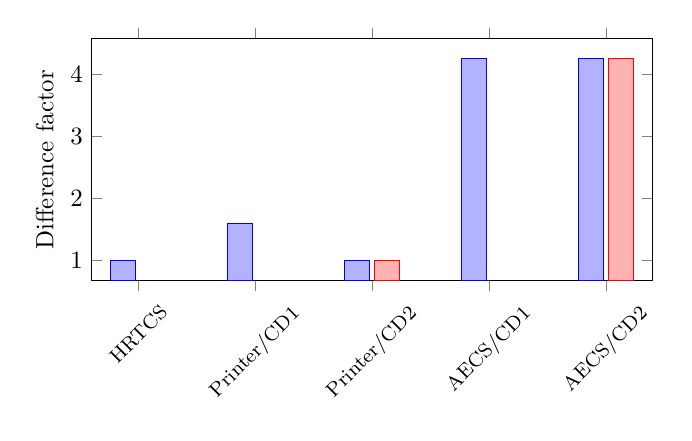
\begin{tikzpicture}[scale=0.9]
	\begin{axis}[
			ybar,xtick=data,
			symbolic x
			coords={HRTCS,Printer/CD1,Printer/CD2,AECS/CD1,AECS/CD2},
			height=5cm,
			width=9.5cm,
%      xlabel=Benchmark,
			x tick label style={rotate=45,font=\footnotesize},
			ylabel=Difference factor,
		]
			\addplot coordinates {(HRTCS,1)(Printer/CD1,1.6)(Printer/CD2,1)(AECS/CD1,4.25)(AECS/CD2,4.25)};
			\addplot coordinates {(Printer/CD2, 1)(AECS/CD2, 4.25)};
	\end{axis}
\end{tikzpicture}
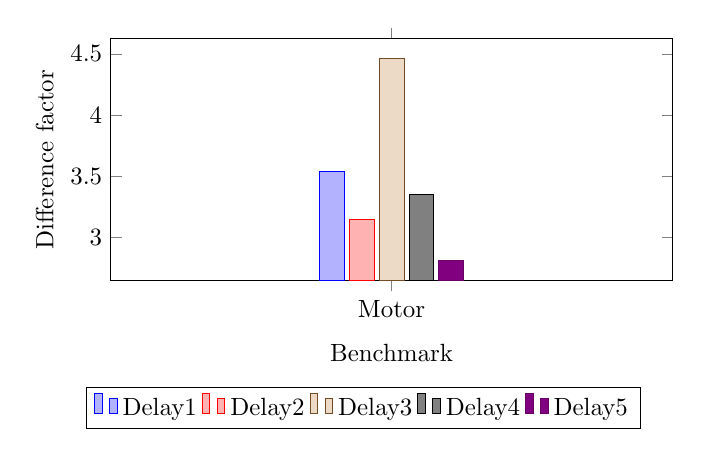
\begin{tikzpicture}[scale=0.9]
	\begin{axis}[
			ybar,xtick=data,
			symbolic x
			coords={Motor},
			height=5cm,
			width=9.5cm,
			xlabel=Benchmark,
			xlabel shift={4pt},
			ylabel=Difference factor,
			legend style={
				anchor=north,
				at={(0.45,-0.44)},
				legend columns=-1,
			}
%      nodes near coords
		]
			\addplot coordinates {(Motor, 3.54)};
			\addplot coordinates {(Motor, 3.15)};
			\addplot coordinates {(Motor, 4.46)};
			\addplot coordinates {(Motor, 3.35)};
			\addplot coordinates {(Motor, 2.81)};
			\legend{Delay1,Delay2,Delay3,Delay4,Delay5}
	\end{axis}
\end{tikzpicture}
\caption{Accuracy of the results}
\label{fig:graph}
\end{figure}

% HRTCS, as already illustrated in Section \ref{sec:intr-motiv}, tests for an
% ability of one's responsiveness by generating green lights between the
% real-time range \emph{M - N}. For AECS \ref{} we have replaced the external
% timer with our delay constructs. Stepper motor controller is originally
% introduced in \cite{Bourke2009a} which converted into SystemJ.

% As one can see in Figure \ref{fig:comparison}, BCRT and WCRT of overall programs
% are smaller when they run on TP-JOP. For example, WCRT and BCRT of HRTCS are
% \(\times\)11.9 and \(\times\)3.4 smaller, respectively, for TP-JOP (0.0028,
% 0.0329 ms) compared to JOP (0.0334, 0.1120 ms). On the other hand, required
% logical delays \emph{d} are generally bigger on TP-JOP e.g. \(\times\)4.5 -
% \(\times\)5.9 and \(\times\)30.9 in Motor and Robot respectively. It is expected
% as their BCRT and WCRT differences are bigger on TP-JOP.
% This also led to greater increase in minimum upper real-time bounds \emph{N} for
% TP-JOP in every example.
% In AECS, there are two clock-domains using delay constructs that each has their
% own BCRT and WCRT. Again, individual BCRT and WCRT is smaller whereas \emph{d}
% is bigger on TP-JOP. One important property to note here, is that BCRT and WCRT
% of any clock-domains are invariant of \emph{d} as explained in Section
% \ref{sec:intr-real-time}. It is our fundamental assumption to find \emph{d} in
% our benchmark programs.
% >>>>>>> 4bffc4b1a43388f5ebf6cc737b9d3b246ee77dc7



%%% Local Variables: 
%%% mode: latex
%%% TeX-master: "paper"
%%% End: 
